%---CAPITULO DOCUMENTADO CON PAUTAS Y PIJOTERÍAS DE ESTILO

%Generalidades:
%--Usar los entornos predefinidos en el style para teoremas y demás.
%--Cuanto más cosas se etiqueten mejor.
%--Nunca usar \\ para saltar de línea, en su lugar, dar a ENTER dos veces.
%--Redactar.
%Cuidado al usar interiores pues es algo que lamentablemente jode el interlineado. Usar el comando reducido \inter cuando se quiera poner un abierto en medio del texto.

%Para este capítulo se usará la abreviatura "etop".
\chapter{Espacios topológicos}
%Todo capítulo será etiquetado con una abreviatura especificada al inicio del archivo.
\label{etop}
%Todo capítulo comienza con una breve introducción, ya sea a modo de breve motivación o a modo de resumen de contenidos (o ambas).
La necesidad del estudio de la proximidad y continuidad, de la forma más abstracta posible, (absteniéndose del uso de la noción de distancia) dio origen a la Topología.

La idea de espacio topológico se comenzó a desarrollar durante los siglos XIX y XX por matemáticos como Fréchet, Kuratowski, Alexandroff y Hausdorff entre otros.

La definición inicial de estos espacios se puede encontrar en el libro \tb{\ti{``Grundzüge der Mengenlehre''}}\footnote{``Teoría abstracta de conjuntos'', publicado en $1914$ por \tb{\ti{Félix Hausdorff}}(1868-1942).} publicado por este último autor.


Al comienzo de este capítulo introducimos la noción moderna de espacio topológico, añadiendo unos cuantos ejemplos, y posteriormente, presentaremos los conjuntos abiertos y cerrados y sus relaciones.%Continuará...
\section{Espacios topológicos. Definición y ejemplos.}
%Etiquetaremos tanto secciones como subsecciones.
\label{etop_definicionEjemplos}
%Es recomendable redactar un poco entre entorno y entorno y soltar un chascarrillo de vez en cuando para dejar reflexionar al lector y que no le parezca un ladrillo.
Comenzamos, como no podía ser de otra manera, definiendo la estructura sobre la que trabajaremos a lo largo de todas estas notas, los llamados espacios topológicos.
%Es recomendable titular cada entorno entre corchetes.
\begin{defi}[Espacio topológico]
	%Cada vez que comencemos un entorno potencialmente referenciable deberá ser etiquetado siguiendo un convenio similar a este.
	\label{etop_def_espacioTopologico}
	%Cada vez que introduzcamos un concepto nuevo es recomendable ponerlo en negrita y cursiva, se puede hacer usando estos comandos, probablemente haya que crear uno más corto porque la verdad que es un poco coñazo.
	Un \tb{\ti{espacio topológico}} es un conjunto arbitrario no vacío $\mc{X}$ equipado con una colección $\T$ de subconjuntos $\mc{U}\subset\mc{X}$ que cumplen las siguientes propiedades:
	%Cuando se está en un entorno es recomendable poner algo de texto antes de un enmerate para que quede mejor.
	\begin{enumerate}
		%Cuando se definen axiomas importantes en el enumerate se sustituyen los números por cosas que llaman la atención (se suele hacer muy pocas veces).
		\item El vacío y el total están en la colección $\T$, es decir, $\{\emptyset, \X\} \subset \T$
		\item La unión arbitraria de conjuntos de $\T$ está en $\T$. Escrito de forma más rigurosa, pero desde luego, menos elegante, 
		$\bigcup_{i\in I}\U_i\in\T$ donde cada $\U_i\in\T$.
		\item La intersección finita de conjuntos de $\T$ está en $\T$. O, dicho de otra forma, $\bigcap_{i=1}^{n}\U_i\in\T$ donde cada $\U_i\in\T$.
	\end{enumerate}
	A menudo hablaremos tan solo de \tbi{espacio} para referirnos a los espacios topológicos.
\end{defi}
%Siempre viene bien algún chascarrillo para liberar tensiones.
Hagamos un par de pequeñas observaciones antes de continuar con nuestro recién empezado viaje cósmico--topológico.
\begin{obs}[Sutilezas]
	\label{etop_obs_sutilezas}
	Se desprende de la definición \ref{etop_def_espacioTopologico} que un espacio topológico no es más que un par $(\X, \T)$. Como es natural, salvo que sea necesario, nos referiremos a un espacio topológico por el conjunto que lo conforma, al igual que hacemos en casi todas las ramas de las matemáticas (espacios vectoriales, grupos, anillos,...).
\end{obs}
Introducimos ahora un poco de terminología con la que el lector no tiene más remedio que hacerse familiar.
\begin{obs}[Terminología]
	\label{etop_obs_terminologia}
	A la familia de conjuntos $\T$ que conforman un espacio topológico $\X$ se le denomina \tbi{topología} de $\X$.
	
	Asimismo, los conjuntos que constituyen los elementos de $\T$ reciben el nombre de \tbi[conjunto!abierto]{abiertos} de $\X$. Normalmente los denotaremos con las letras $\U$ o $\W$.
	
	Como es natural, nos referiremos a los elementos de $\X$ como \tbi[punto]{puntos}.
\end{obs}
Introducimos ahora unos pocos ejemplos para irnos familiarizando con el concepto de espacio topológico viendo lo general que puede llegar a ser.
\begin{exa}[Topologías]
	\label{etop_exa_topologias}
	Las demostraciones de que, efectivamente, se cumplen las restricciones impuestas por la definición \ref{etop_def_espacioTopologico}, o bien ya se han hecho en cursos anteriores, o bien se dejan al lector como ejercicio inmediato.
	\begin{enumerate}
		\item Un espacio métrico $(M,d)$ es un espacio topológico con la topología definida por los conjuntos abiertos en el sentido de los espacios métricos, es decir
		%Se pone una estrellita para que no introduzca número, si no ponemos la estrellita debemos etiquetar la ecuación.
		\begin{equation}
		\label{etop_eq_topologiaRn}
		\T = \{\U\subset M\midc \forall x\in\U\ \exists\  \bola_{d}(x,\varepsilon)\subset\U\}
		\end{equation}
		A esta topología la llamamos \tbitop[$\T_u$]{usual} o inducida por la métrica.
		\item Una topología interesante por su simpleza, y por que dota a cualquier conjunto no vacío $\X$ con estructura de espacio topológico, es la llamada \tbitop[$\T_t$]{trivial}, que viene definida por \begin{equation}
		\label{etop_eq_topologiaTrivial}
		\T=\{\emptyset, \X\}
		\end{equation}
		\item Siguiendo la idea del ejemplo anterior, pero a la inversa, encontramos una topología que también dota de estructura topológica a cualquier conjunto no vacío $\X$. Esta topología viene dada por
		\begin{equation}
		\label{etop_eq_topologiaDiscreta}
		\T = \partes(\X)
		\end{equation}
		A esta topología la llamaremos \tbitop[$\T_d$]{discreta}.
		
		\begin{figure}[h!]
			\centering
			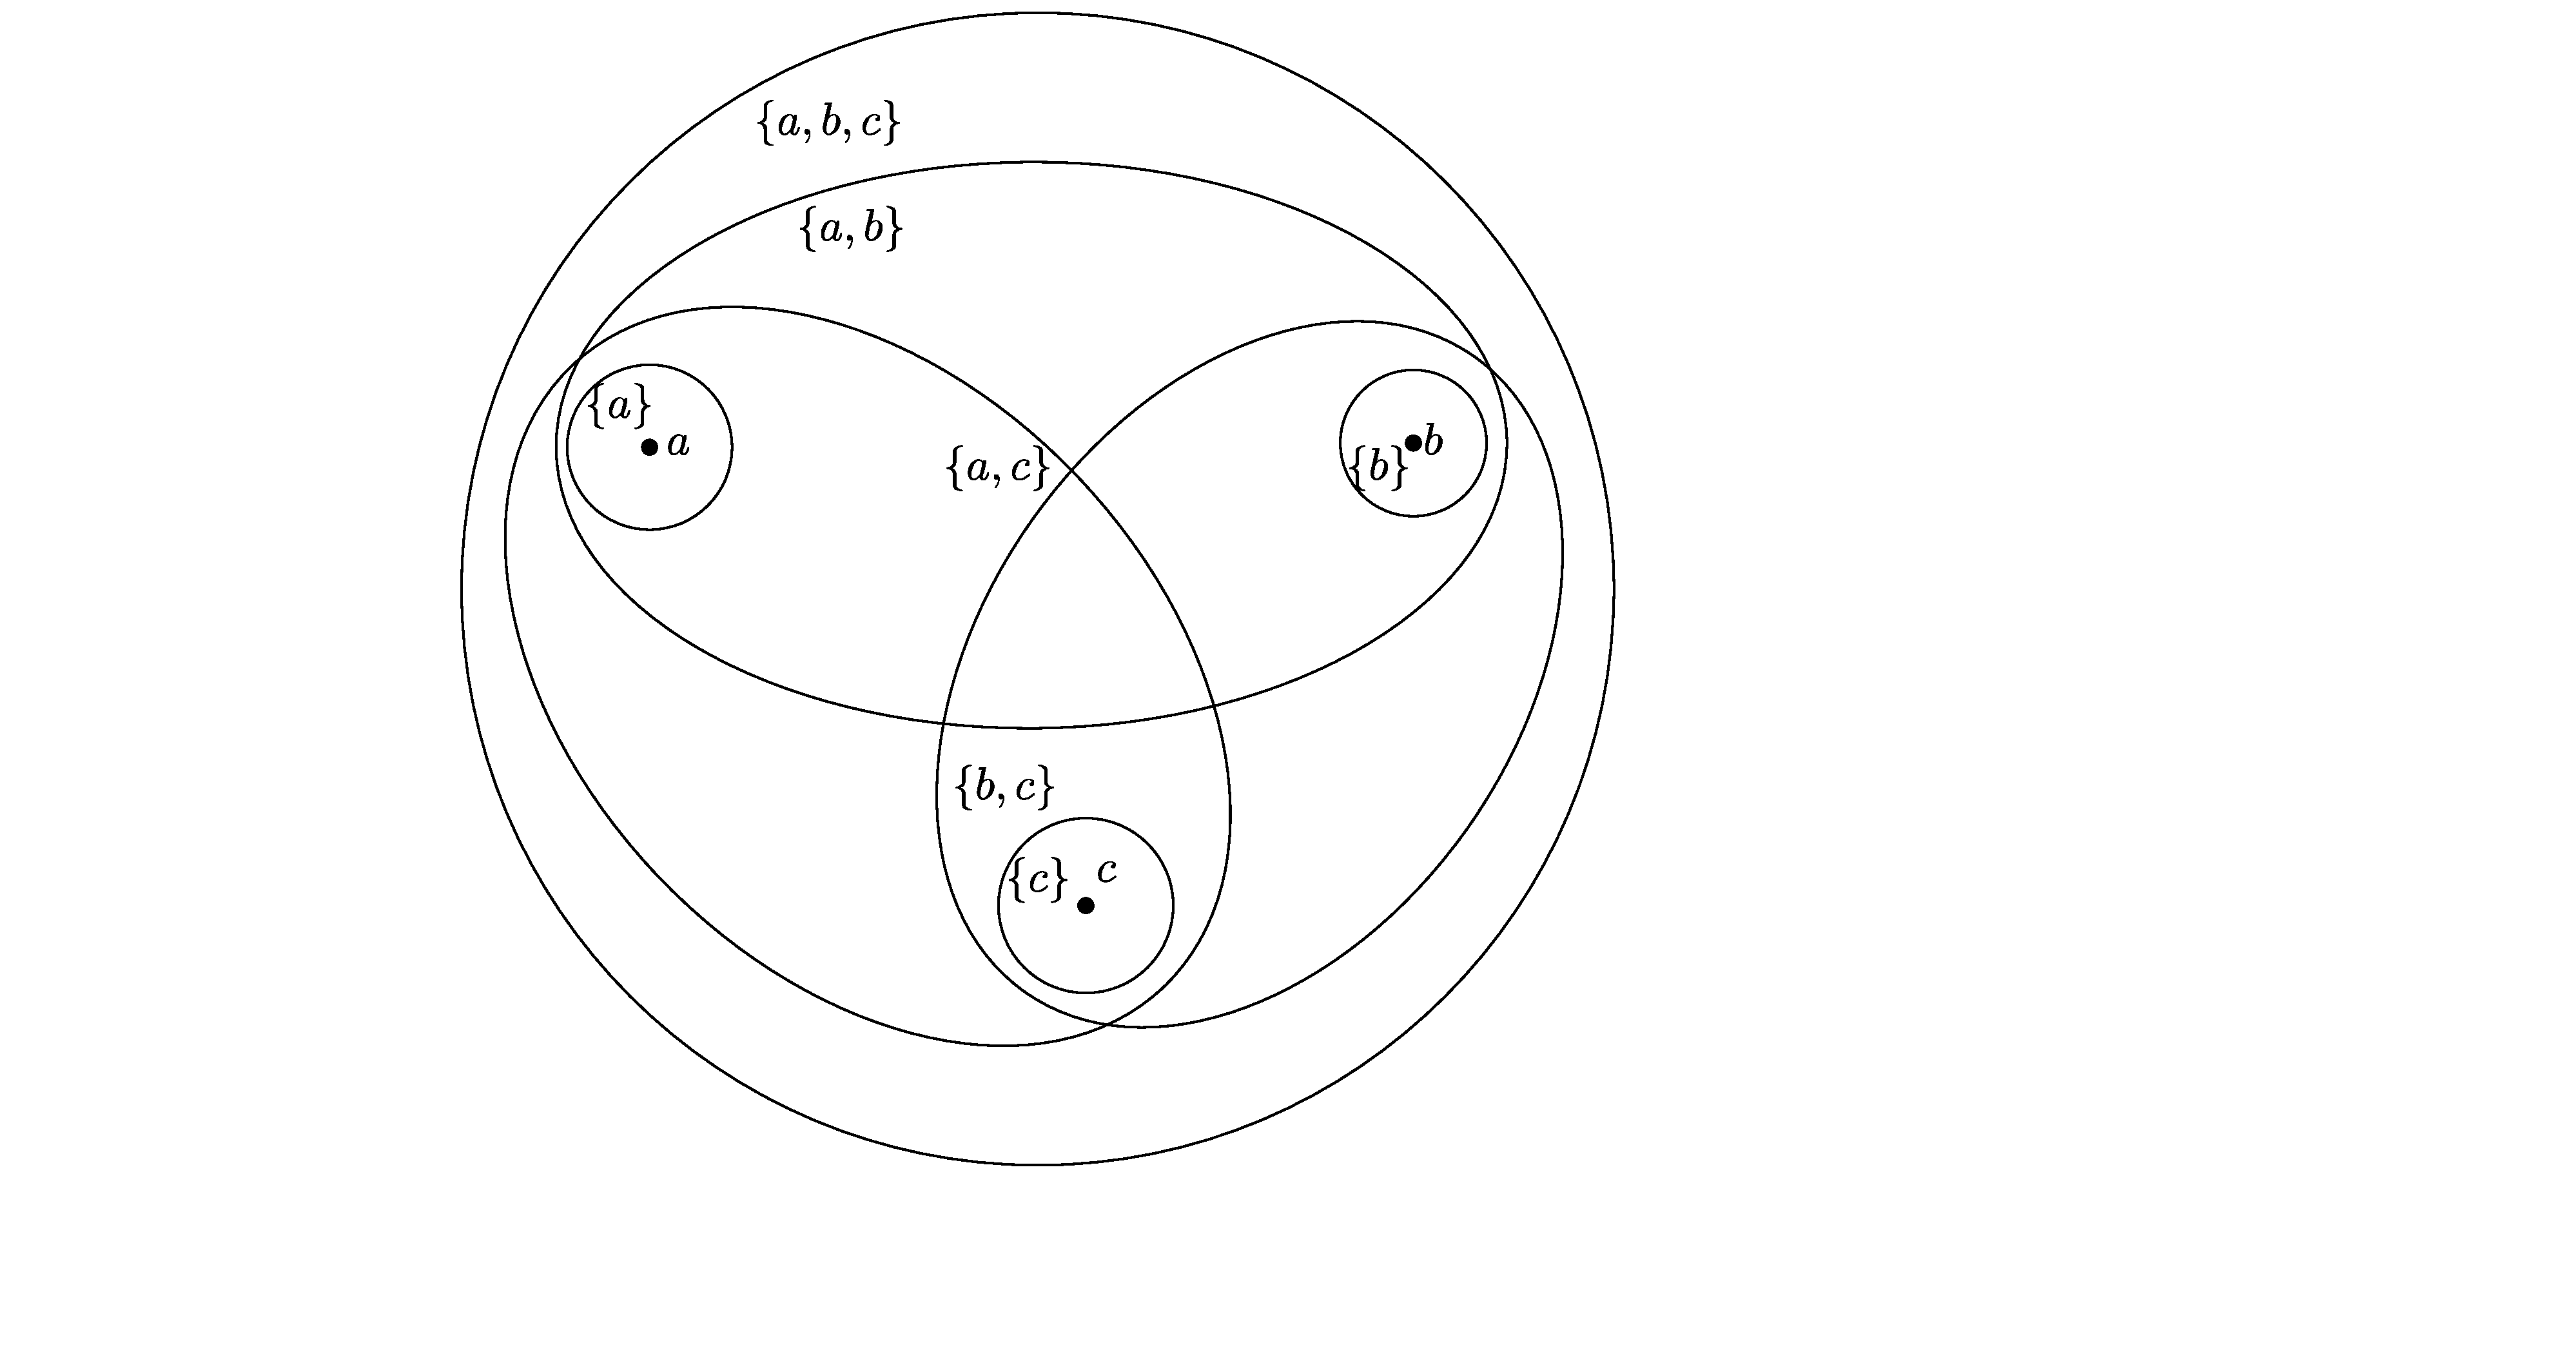
\includegraphics[scale = 0.25]{img/TopologiaDiscreta}
			\caption{Ilustración de la topología discreta para un conjunto de tres puntos.}
			\label{etop_img_discr}
		\end{figure}
		
		\item Como último ejemplo curioso nos queda la llamada \tbitop{del punto}. Consiste en considerar como abiertos a todos los subconjuntos de un conjunto $\X$ que contengan a un determinado punto $a$. Es decir
		\begin{equation}
		\label{etop_eq_topologiaPunto}
		\T_a = \{\U \subset \X\midc a\in\U\}\cup\{\emptyset\}
		\end{equation}
		
		\begin{figure}[h!]
			\centering
			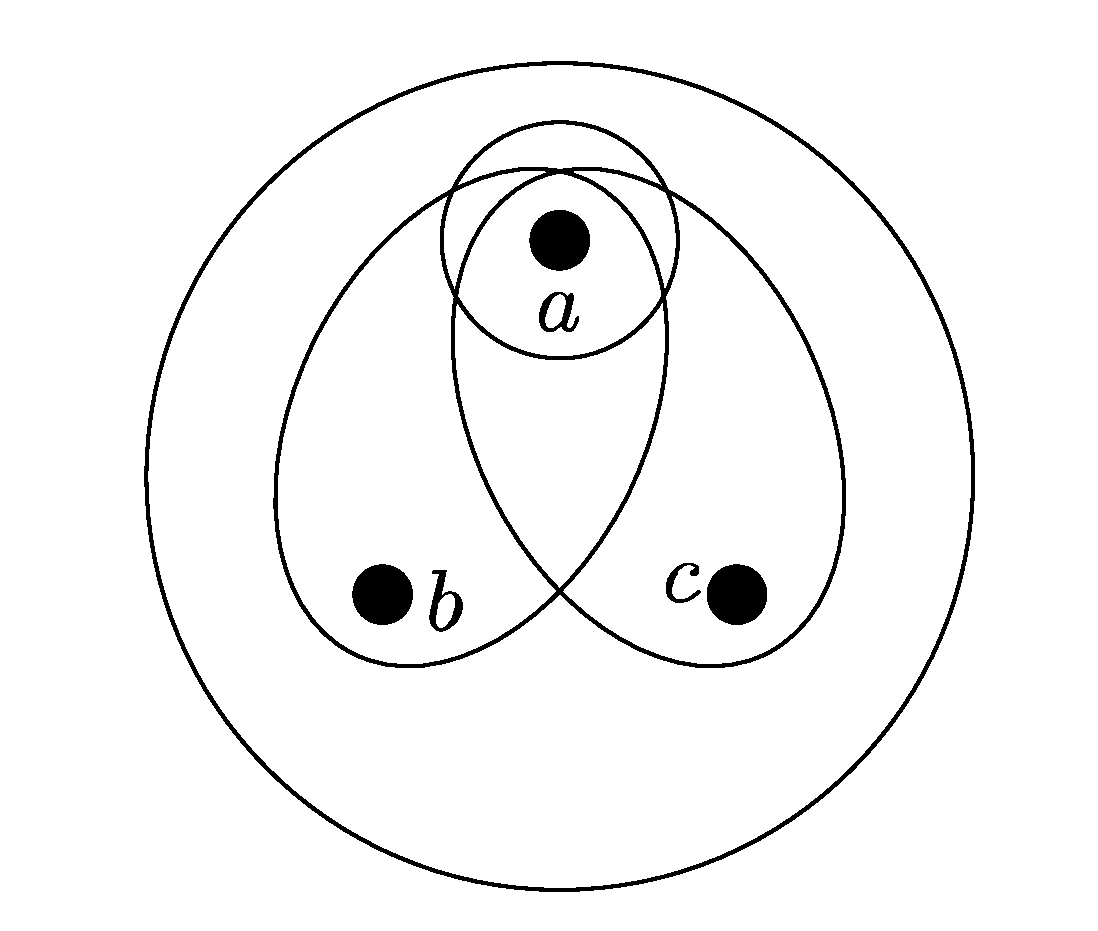
\includegraphics[scale = 0.25]{img/TopologiaPunto}
			\caption{Ilustración de la topología del punto para un conjunto de tres puntos.}
			\label{etop_img_punto}
		\end{figure}
		
		%Comento este ejemplo porque no se entiende un zipote lo que explicó este señor.
		
		%\item Como topología especial y rara, tomemos cuatro puntos a, b, c, d, siendo a y b cerrados, y c y d abiertos. Este espacio topológico es homótopo a la circunferencia $(S^{1})$ (viendo así que los conjuntos finitos pueden ser muy interesantes, aunque de primeras no nos lo imaginemos).
	\end{enumerate}
	Con lo que ya tenemos una gama lo suficientemente amplia de ejemplos como para ir tirando.
\end{exa}
Para finalizar la sección observamos que en un mismo conjunto $\X$ podemos definir diversas topologías. Dichas topologías pueden ``compararse'' en determinado contexto.
\begin{defi}[Relación de orden entre topologías]
	Consideremos $\T$ y $\T'$ dos topologías definidas sobre un conjunto $\X$.
	
	Si se verifica que $\T \subset \T'$ diremos que $\T$ es más \tbi[topología más gruesa]{gruesa} que $\T'$ y que $\T'$ es más \tbi[topología más fina]{fina} que $\T$.
\end{defi}
En lo que resta de capítulo iremos introduciendo algunos conceptos generales de los que haremos uso de forma constante a lo largo del curso.
\section{Conjuntos abiertos e interior}
\label{etop_entornos}
En esta sección introducimos el concepto de entorno, cuya utilidad inmediata es caracterizar a los conjuntos abiertos de un espacio topológico $\X$.
\begin{defi}[Entorno de un punto]
	\label{etop_def_entorno}
	Un \tbi{entorno} de un punto $a\in\X$ es un conjunto que contiene a un abierto que contiene al punto $a$.
\end{defi}
Normalmente denotaremos con la letra $\V$ a los entornos, esta costumbre se debe a un galicismo. %¿cuál?

Escribamos la definición de entorno \ref{etop_def_entorno} de forma conjuntista para que no quede ninguna duda.

Dado $\V\subset \X$, se dice entorno de $a\in \X$ si existe un abierto $\U$ de forma que
\begin{equation}
\label{etop_eq_entorno}
a\in\U\subset\V
\end{equation}

Como ya adelantamos, se puede usar la noción de entorno para caracterizar a los abiertos, tal y como muestra el siguiente lema, que será usado sin cesar a lo largo de estas notas.
\begin{lem}[Caracterización de abiertos]
	\label{etop_lem_caracterizacionAbiertos}
	$\U$ es abierto si y solo si es entorno de todos sus puntos.
\end{lem}
\begin{proof}
	Supongamos que $\U$ es abierto, entonces, dado un punto $a\in\U$ es evidente que $\U$ contiene a un abierto (él mismo) que contiene al punto $a$. Luego $\U$ es, trivialmente, entorno de todos sus puntos.
	
	Recíprocamente, si $\U$ es entorno de todos sus puntos, entonces, para cada punto $a\in\U$ se cumple que
	\begin{equation*}
	a\in\U_a\subset\U
	\end{equation*}
	de donde se desprende que
	\begin{equation*}
	A:=\bigcup_{a\in\U}\U_a\subset\U
	\end{equation*}
	Más aún, se da la otra contención, y además, de forma trivial, ya que todo punto de $\U$ pertenece a algún $\U_a$, luego también a la unión de todos. Luego
	\begin{equation*}
	\U=A
	\end{equation*}
	Como la unión arbitraria de abiertos es abierto, $A$ es abierto, con lo que se sigue el resultado.
\end{proof}
En general, un conjunto será entorno de algunos de sus puntos, en principio no de todos. De esta idea surge la siguiente definición.
\begin{defi}[Punto interior]
	\label{etop_def_puntoInterior}
	Dado un conjunto $A\subset\X$, diremos que un punto $a\in\X$ es un \tbi[punto!interior]{punto interior} de $A$ si $A$ es entorno de $a$.
\end{defi}

Esto pretende modelizar matemáticamente la idea de ``estar muy metido dentro de algo''.

Será algo habitual de ahora en adelante tratar de determinar el conjunto de puntos interiores de un determinado conjunto $A\subset\X$, a este conjunto se le denomina \tbi{interior} de $\X$.

Antes de continuar, fijemos unas cuantas notaciones que utilizaremos según el contexto para referirnos al interior de un conjunto.
\begin{equation}
\label{etop_eq_notacionInterior}
\Int_{\X}(A)=\inter{A}=\Int(A)
\end{equation}
Merece la pena notar que el interior de un conjunto puede ser el conjunto vacío, así como que trivialmente se da la desigualdad conjuntista
\begin{equation}
\label{etop_eq_desigualdadInterior1}
\inter{A}\subset A
\end{equation}
Veamos ahora unos resultados elementales, pero a la vez cruciales, del interior de un conjunto.
\begin{lem}[Apertura del interior]
	\label{etop_lem_aperturaInterior}
	El interior de un conjunto $A$ es un abierto.
\end{lem}
\begin{proof}
	Para probar esto haremos uso del lema \ref{etop_lem_caracterizacionAbiertos}, es decir, trataremos de ver que es entorno de todos sus puntos.
	
	En efecto, dado un punto $a\in\inter{A}$, existe un abierto $\U_a\subset A$ de manera que $a\in\U_a$. Luego para ver que $\inter{A}$ es un entorno de $a$ basta demostrar la inclusión $\U_a\subset\inter{A}$, hagámoslo.
	
	Sea $x\in\U_a\subset A$, es claro que $A$ es entorno de $x$, luego $x\in\inter{A}$.
	
	Con lo cual hemos demostrado que $\inter{A}$ es entorno de todos sus puntos.
\end{proof}

El otro resultado elemental que caracteriza al interior de un conjunto $A$, es que es el mayor abierto contenido en $A$.

Presentamos aquí los primeros pasos de la demostración por ser especialmente útiles y omnipresentes en las matemáticas en general.

Como la unión de abiertos es abierto, es claro que una forma de construir el mayor abierto contenido en cierto conjunto es, coleccionar los abiertos contenidos en dicho conjunto y unirlos. Escrito formalmente, tomamos el conjunto
\begin{equation}
\label{etop_eq_mayorAbierto}
B:=\bigcup_{\W\subset A}\W\text{ con $\W$ abierto.}
\end{equation}
Es claro que $B\subset A$, ya que es una unión de conjuntos contenidos en $A$, además, si hubiera un abierto más grande contenido en $A$ que $B$, este pertenecería a la familia de conjuntos que estamos uniendo, lo cual es absurdo.

Presentamos el final de la demostración en forma de lema.
\begin{lem}[Caracterización del interior]
	\label{etop_lem_caracterizacionInterior}
	El interior de un conjunto $A$ es el mayor abierto contenido en $A$.
\end{lem}
\begin{proof}
	Por el lema \ref{etop_lem_aperturaInterior} sabemos que $\inter{A}$ es abierto, luego, por la ecuación \eqref{etop_eq_mayorAbierto} solo queda probar la igualdad
	\begin{equation*}
	\inter{A}=\bigcup_{\W\subset A}\W\subset A
	\end{equation*}
	Y esto es prácticamente trivial. Veámoslo.
	
	Por una parte, $\inter{A}$ es un abierto contenido en $A$, luego está contenido en la unión de los abiertos contenidos en $A$.
	
	Por otra parte, dado $x\in\bigcup_{\W\subset A}\W$, es claro que, como $\bigcup_{\W\subset A}\W\subset A$ es un abierto, $A$ es entorno de $x$, luego $x\in\inter{A}$, lo que concluye la demostración.
\end{proof}

El lema \ref{etop_lem_caracterizacionInterior} es bastante fuerte y produce algunos corolarios interesantes que presentamos a modo de observaciones.
\begin{obs}[Propiedades del interior]
	\label{etop_obs_propiedadesInterior}
	Enumeramos algunas propiedades del interior.
	\begin{enumerate}
		\item El interior del interior de un conjunto es el interior de dicho conjunto. Si lo escribimos sin que suene como un trabalenguas tenemos
		\begin{equation}
		\label{etop_eq_dobleInterior}
		\inter{\inter{A}}=\inter{A}
		\end{equation}
		Esto es trivial ya que al ser $\inter{A}$ un abierto, el mayor abierto contenido en él es él mismo.
		\item Un conjunto es abierto si y solo si coincide con su interior, es decir
		\begin{equation}
		\label{etop_eq_abiertoInterior}
		A=\inter{A}
		\end{equation}
		Esto es cierto por la misma razón que lo es la ecuación \eqref{etop_eq_dobleInterior}.
		\item Los interiores preservan las contenciones. O lo que es lo mismo
		\begin{equation}
		\label{etop_eq_interiorContencion}
		A\subset B\ra \inter{A}\subset\inter{B}
		\end{equation}
		Por la desigualdad \eqref{etop_eq_desigualdadInterior1} es claro que $\inter{A}\subset B$, y como $\inter{B}$ es el mayor abierto contenido en $B$, y $\inter{A}$ es un abierto contenido en $B$, es claro que $\inter{A}\subset\inter{B}$.
	\end{enumerate}
	Esto ya nos da cierta artillería para defendernos con estos conjuntos.
\end{obs}
Con esto podemos decir que ya hemos liquidado todo lo referente a conjuntos abiertos.
\section{Conjuntos cerrados y adherencia}
\label{etop_cerradosAdherencia}
En esta sección estudiaremos los conjuntos cerrados.

Cabe destacar que la noción de ser cerrado no es exactamente la contraria a la de ser abierto, ya que, como veremos más adelante, hay conjuntos que no son ni abiertos ni cerrados así como conjuntos que son abiertos y cerrados a la vez.

\begin{defi}[Conjunto cerrado]
	Un conjuto $\F$ de un espacio topológico $\X$ se dice \tbi[conjunto!cerrado]{cerrado} si su complementario, $\X\setminus\F$, es abierto.
\end{defi}

Usualmente denotaremos a los conjuntos cerrados con las letras $\F$ o $\mc{H}$.

Usando propiedades básicas de teoría de conjuntos (leyes de DeMorgan, distributividad,\dots) se obtienen algunas propiedades elementales de los conjuntos cerrados.
\begin{lem}[Propiedades de los cerrados]
	\label{etop_lem_propiedadesCerrados}
	Dado un espacio topológico $\X$ se verifica
	\begin{enumerate}
		\item El vacío y el total son cerrados.
		\item La intersección arbitraria de cerrados es cerrada.
		\item La unión finita de cerrados es cerrada.
	\end{enumerate}
\end{lem}
\begin{proof}Vayamos caso por caso.
	\begin{enumerate}
		\item $\X$ es cerrado pues $\X\setminus\X=\emptyset$ es abierto.
		
		Asimismo, $\emptyset$ es cerrado pues $\X\setminus\emptyset=\X$ es abierto.
		\item $\bigcap_{i\in I}\F_i$ es cerrado ya que, aplicando las leyes de DeMorgan
		\begin{equation*}
		\X\setminus\left(\bigcap_{i\in I}\F_i\right)=\bigcup_{i\in I}\X\setminus\F_i
		\end{equation*}
		es abierto por ser la unión arbitraria de abiertos un abierto.
		\item $\bigcup_{i=1}^n\F_i$ es cerrado, basta tomar el complementario y ver que es abierto por ser intersección finita de abiertos.
		\begin{equation*}
		\X\setminus\left(\bigcup_{i=1}^{n}\F_i\right)=\bigcap_{i=1}^n\X\setminus\F_i
		\end{equation*}
	\end{enumerate}
	Con lo que concluye la demostración.
\end{proof}
\begin{obs}[Abiertos y cerrados a la vez]
	\label{etop_obs_abiertoCerrado}
	Basta con mirar con atención este lema \ref{etop_lem_propiedadesCerrados} para darse cuenta de que hemos encontrado dos conjuntos que son abiertos y cerrados a la vez, el vacío y el total.
	
	Estos conjuntos abiertos y cerrados a la vez (o ``\tbi[clopen]{clopens}'', del inglés close--open) son de vital importancia a la hora de estudiar la conexión, como veremos más adelante. 
\end{obs}
%----DEJO ESTO COMENTADO HASTA QUE SE DE LA DEFINICIÓN DE COMPACTO----
%Una breve anotación que nos será útil en el futuro. Para la comprobación de compacidad en un computo, nos será útil la utilización de cerrados. Veamos un ejemplo, introducido para motivar esta observación.\\
%\textbf{\underline{Ejemplo}}\\
%\\
%$\cx = \bigcup_{i \in I}\cup_{i} \Rightarrow \cx = \cu_{i_{1}} \cup \ldots \cup \cu_{i_{k}}$ por definición de compacto, que se verá más adelante. Pasando a complementarios tenemos:\\
%$\emptyset = \bigcap_{i \in I}\cf_{i} \Rightarrow \emptyset = \cf_{i_{1}} \cap \ldots \cap \cf_{i_{k}}$.\\
%Por lo tanto para ser compacto el conjunto, la unión de cerrados pertenecientes al conjunto finita a de ser el vacío.\\
%Veamos un caso en el que no se cumple:\\
%$\emptyset = \bigcap(0,\frac{1}{n}] \subset (0,\infty)$. Estos conjuntos son cerrados en este espacio. Pero observamos trivialmente que cualquier $n_0$ finito que coja, la intersección va a dar no vacía, luego el conjunto no es compacto.
%----FIN----
Introducimos ahora un concepto elemental pero interesante, el concepto de puntos adherentes y adherencia.
\begin{defi}[Punto adherente]
	\label{etop_defi_puntoAdherente}
	Un punto $a\in\X$ se dice \tbi[punto!adherente]{adherente} a un conjunto $A\subset\X$ si todo entorno de $a$ corta al conjunto $A$.
	
	Esta definición pretende modelizar la idea de estar ``muy pegado'' a algo.
\end{defi}

\begin{obs}[Definición equivalente]
	\label{etop_defi_equivalente}
	Podríamos haber sustituido la definición \ref{etop_defi_puntoAdherente} por una igual pero cambiando la palabra entorno por la palabra abierto.
	
	La comprobación de que esto se puede hacer es inmediata y se deja al lector.
\end{obs}
Como ya es habitual, coleccionaremos los puntos adherentes a un conjunto dado y estudiaremos las propiedades del conjunto de puntos adherentes. Introduzcamos una definición para verlo formalmente.
\begin{defi}[Adherencia]
	\label{etop_defi_adherencia}
	Se define la \tbi{adherencia} o \tbi{clausura} de un conjunto $A\subset\X$ como el conjunto de los puntos adherentes de $A$.
\end{defi}

Usualmente denotaremos a la adherencia de alguna de las siguientes formas
\begin{equation}
\label{etop_eq_adherencia}
\Adh_{\X}(A)=\Adh(A)=\adher{A}
\end{equation}

Vamos a desgranar ahora una serie de resultados que nos van a hacer ver que adherencia e interior de un conjunto son, de alguna manera, conceptos duales.

Comenzamos en primer lugar con algo casi trivial.
\begin{obs}[Adherencia y conjunto]
	\label{etop_obs_adherenciaConjunto}
	Es claro que se verifica que
	\begin{equation}
	\label{etop_eq_adherenciaConjunto}
	A\subset\adher{A}
	\end{equation}
	Esto es debido a que, evidentemente, cualquier entorno de $a$ contiene al punto $a$, luego, por definición, corta al conjunto $A$.
	
	Visto en perspectiva, esta desigualdad es de alguna manera la dual a la \eqref{etop_eq_desigualdadInterior1}.
	
	Además, combinando ambas desigualdades obtenemos que un conjunto siempre queda ``ensandwichado'' entre su interior y su adherencia.
	\begin{equation*}
		\inter{A}\subset A\subset\adher{A}
	\end{equation*}
	Lo cual puede resultar de utilidad.
\end{obs}

\begin{lem}[Clausura de la adherencia]
	\label{etop_lem_clausuraAdherencia}
	La adherencia de un conjunto $A$ es un cerrado.
\end{lem}
\begin{proof}
	Usaremos lo único que tenemos, es decir, la definición de conjunto cerrado. Por ende, probaremos que $\X\setminus\adher{A}$ es abierto, para lo cual veremos que es entorno de todos sus puntos, haciendo buen uso del lema \ref{etop_lem_caracterizacionAbiertos}.
	
	Dado $x\in\X\setminus\adher{A}$, como $x$ no es un punto adherente, entonces existirá un entorno $\V(\ni x)$, el cual podemos escoger abierto sin pérdida de generalidad tal que se verifica
	\begin{equation*}
	\V\cap A=\emptyset
	\end{equation*}
	Si consiguiéramos demostrar que se de la igualdad
	\begin{equation*}
	\V\cap \adher{A}=\emptyset
	\end{equation*}
	habríamos acabado ya que tendríamos que $x\in\V\subset\X\setminus\adher{A}$, que es, por definición que $\X\setminus \adher{A}$ sea entorno de $x$.
	
	En efecto, la comprobación de esta igualdad es muy fácil, ya que, si tomamos un $y\in\V$, al ser $\V$ abierto, es entorno de $y$.
	
	Por tanto, tendríamos que el punto $y$ no es adherente, ya que existe un entorno, el propio $\V$ que no corta con el conjunto $A$, incumpliendo así la definición \ref{etop_defi_puntoAdherente}.
\end{proof}
Continuamos esta dualización de conceptos dándonos cuenta de que la adherencia es el menor cerrado que contiene a $A$. Como antes, parte de la demostración se basa en un procedimiento estándar que pasamos a explicar.

Es fácil darse cuenta de que, como la intersección arbitraria de cerrados es un cerrado, el menor conjunto cerrado que contiene a uno dado puede ser construido de la siguiente manera
\begin{equation}
\label{etop_eq_menorCerrado}
B:=\bigcap_{\mc{H}\supset A}\mc{H}
\end{equation}
En efecto es un conjunto que contiene a $A$ ya que todos los conjuntos de la familia a intersecar contienen a $A$, además, es el menor de ellos, ya que, de haber uno más pequeño, pertenecería a la familia que se está intersecando, lo cual es absurdo (¡compruébese!).

Presentamos, otra vez, en forma de lema, el resto de la demostración.
\begin{lem}[Caracterización de la adherencia]
	\label{etop_lem_caracterizacionAdherencia}
	La adherencia de un conjunto $A$ es el menor cerrado que contiene a $A$.
\end{lem}
\begin{proof}
	Por la ecuación \eqref{etop_eq_menorCerrado} la demostración se reduce a comprobar que
	\begin{equation*}
	\adher{A}=\bigcap_{\mc{H}\supset A}\mc{H}
	\end{equation*}
	Y esto es una comprobación inmediata.
	
	Por un lado, como $\adher{A}$ es un cerrado que contiene a $A$, es claro que $\adher{A}$ se encuentra en la familia a intersecar, luego contiene a la intersección de la familia.
	
	Recíprocamente, dado un punto adherente $x$, si hubiera un conjunto $\mc{H}$ de la familia tal que $x\not\in \mc{H}$, entonces tendríamos que $x\in\X\setminus\mc{H}\subset\X\setminus A$.
	
	Como $\mc{H}$ es cerrado, $\X\setminus\mc{H}$ es abierto, y, por tanto existirá un entorno $\V$ de $x$ de manera que \begin{equation*}
	x\in\V\subset\X\setminus\mc{H}\subset\X\setminus A
	\end{equation*}
	
	Y, por ende, $\V\cap A=\emptyset$, contra la definición de punto adherente.
\end{proof}
Presentamos a continuación unas cuantas igualdades conjuntistas que pueden resultar bastante útiles al lector.
\begin{prop}[Complementario de la adherencia]
	\label{etop_prop_compAdher}
	\begin{equation*}
	\X\setminus\adher{A}=\Int(\X\setminus A)
	\end{equation*}
\end{prop}
\begin{proof}
	Procedemos por doble contención.
	\begin{enumerate}
		\item[\bsubset] Sea $z\in\X\setminus\adher{A}$. Como $z$ no es adherente a $A$, por definición \eqref{etop_defi_adherencia} habrá un entorno $\V_z$ de $z$ de manera que $\V_z\cap A=\emptyset$. En particular, podremos extraer un entorno abierto $\U_z$ tal que verifique
		\begin{equation*}
		\U_z\cap A =\emptyset
		\end{equation*}
		Tratamos de demostrar que $z$ es punto interior de $\X\setminus A$, esto es, por definición \eqref{etop_def_puntoInterior}, que $\X\setminus A$ sea entorno de $z$, esto a su vez significa que hay un abierto $\U_z'$ contenido en $\X\setminus A$ de forma que $z\in\U_z'$. Así pues el problema se reduce a encontrar dicho entorno, sin embargo, es trivial comprobar el entorno $\U_z$ anteriormente definido cumple los requisitos.
		\item[\bsupset] Sea $z\in\Int(\X\setminus A)$, demostremos que $z$ no es adherente a $A$, para lo cual debemos encontrar un entorno de $z$, al que llamaremos $\V_z$, de manera que no corte al conjunto $A$. Esto es trivial, ya que $z$ es punto interior de $\X\setminus A$, luego el propio $\X\setminus A$ es entorno de $z$, y, evidentemente, no corta a $A$.
	\end{enumerate}
	Con lo que concluye la prueba.
\end{proof}

Insistiendo es esta dualidad vía complementación entre abiertos y cerrados, presentamos un corolario inmediato.
\begin{cor}[Complementario del interior]
	\label{etop_cor_compInter}
	\begin{equation*}
	\X\setminus\inter{B}=\Adh(\X \setminus B)
	\end{equation*}
\end{cor}
\begin{proof}
	Nos limitaremos a comprobar que ambos conjuntos tienen el mismo complementario. En efecto, por una parte
	\begin{equation*}
	\X \setminus (\X \setminus \inter{B}) = \inter{B}
	\end{equation*}
	Por otro lado, denotando $A:=\X \setminus B$ tenemos
	\begin{equation*}
	\X \setminus \Adh(\X \setminus B)=\X \setminus \adher{A}\stackrel{\textrm{Prp.\ref{etop_prop_compAdher}}}{=}\Int(\X \setminus A)=\Int(\X \setminus (\X \setminus B))=\Int(B)=\inter{B}
	\end{equation*}
	Con lo que se tiene el resultado.
\end{proof}
Una última identidad notable, un poco más profunda que las anteriores es la que relaciona la unión de las adherencias con la adherencia de las uniones.
\begin{prop}[Unión de adherencias]
	La unión de las adherencias es la adherencia de las uniones.
	\label{etop_prop_unionAdher}
	\begin{equation*}
	\adher{A\cup B}=\adher{A}\cup\adher{B}
	\end{equation*}
\end{prop}
\begin{proof}
	Procedemos por doble contención.
	\begin{enumerate}
		\item[\bsubset] 
		Dado $z\in \adher{A\cup B}$, todo entorno $\V_z$ de $z$ corta a $A\cup B$. Veamos que $z$ es, o bien adherente a $A$, o bien adherente a $B$ (quizá a ambos). Para ello supondremos que no es adherente a ninguno de ellos, es decir, que existe un entorno $\W_z$ de $z$ que no corta ni a $A$ ni a $B$. Si este entorno existiera tampoco cortaría a la unión (compruébese), lo cual es absurdo.
		\item[\bsupset]
		Dado un punto $z\in\adher{A}\cup\adher{B}$, veamos que todo entorno de $\V_z$ de $z$ corta a $A\cup B$. Si no lo hiciera, para cada punto $x\in\V_z$, $x$ no estaría en $A$, luego $A\cap \V_z=\emptyset$. Análogamente ocurriría con $B$, lo cual contradice nuestra hipótesis.
	\end{enumerate}
	Con lo que finaliza la demostración.
\end{proof}
\begin{obs}[Demostración alternativa]
	Una demostración alternativa y quizá más contundente de la proposición \ref{etop_prop_unionAdher} consistiría en usar las propiedades de distributividad de las operaciones conjuntistas.
	
	En efecto, $z\in\adher{A\cup B}$ si y solo si todo abierto $\U$ de $z$ cumple que
	\begin{equation*}
		\U\cap(A\cup B)\stackrel{!}{=}(\U\cap A)\cup(\U\cap B)\not=\emptyset
	\end{equation*}
	lo cual es equivalente a decir que o bien $\U\cap A$ o bien $\U\cap B$ son no vacíos, con lo que hemos terminado, es decir $z\in\adher{A}\cup\adher{B}$.
\end{obs}
Por supuesto, este resultado presenta un dual inmediato.
\begin{cor}[Intersección de interiores]
	El interior de la intersección es la intersección de los anteriores.
	\begin{equation*}
	\Int(A\cap B)=\inter{A}\cap\inter{B}
	\end{equation*}
\end{cor}
\begin{proof}
	Comprobaremos, como ya hicimos anteriormente, que ambos conjuntos tienen el mismo complementario.
	
	Por un lado
	\begin{equation*}
	\X \setminus \Int(A\cap B)=\Adh(X\setminus (A\cap B))
	\end{equation*}
	Recíprocamente
	\begin{multline*}
	\X \setminus (\inter{A}\cap \inter{B})=(\X \setminus \inter{A})\cup(\X \setminus \inter{B})=\Adh(\X \setminus A)\cup \Adh(\X \setminus B))=\\=\Adh((\X \setminus A) \cup (\X \setminus B))=\Adh(X\setminus (A\cap B))
	\end{multline*}
	Así, el resultado se sigue.
\end{proof}
El resultado análogo a la proposición \ref{etop_prop_unionAdher} con la intersección no se da, tal y como muestra el siguiente ejemplo.
\begin{exa}[Cuadrados abiertos]
	\label{etop_ejem_cuadradosAbiertos}
	Si consideramos los conjuntos
	\begin{equation*}
	\begin{array}{cc}
	A:=(0,1)\times(0,1)\qquad&\qquad B:=(1,2)\times(0,1)
	\end{array}
	\end{equation*}
	En $\R^2$ con la topología usual, es fácil demostrar (se deja al lector) que $\adher{A\cap B}=\emptyset$ mientras que $\adher{A}\cap\adher{B}=\{1\}\times[0,1]$.
\end{exa}
Vistas todas estas igualdades, al igual que hicimos en la observación \ref{etop_obs_propiedadesInterior}, caractericemos los conjuntos cerrados a partir del concepto de adherencia.
\begin{prop}[Cerrados y adherencia]
	\label{etop_prop_cerradosAdher}
	Un conjunto es $A$ cerrado si y solo si coincide con su adherencia. Es decir
	\begin{equation*}
	A=\adher{A}
	\end{equation*}
\end{prop}
\begin{proof}
	Si $A$ es cerrado, como $\adher{A}$ es el menor cerrado que contiene a $A$, es claro que se tiene que dar la igualdad $A=\adher{A}$.
	
	Recíprocamente, si se da la igualdad $A=\adher{A}$, como $\adher{A}$ es cerrado, también lo será $A$.
\end{proof}
Añadimos una observación final trivial, simplemente por curiosidad.
\begin{obs}[Doble adherencia]
	Dado un conjunto $A$, se tiene que
	\begin{equation*}
	\adher{A}=\adher{\adher{A}}
	\end{equation*}
	Esto es inmediato ya que, como $\adher{A}$ es un cerrado, coincide con su adherencia.
\end{obs}
\section{Puntos de acumulación y conjuntos densos}
En esta sección presentamos el concepto de punto de acumulación, que es muy útil para trabajar con sucesiones, como veremos más adelante. Además, definiremos la idea de que un conjunto sea denso de varias maneras que nos serán muy útiles a la hora de resolver problemas.
\begin{defi}[Punto de acumulación]
	\label{etop_defi_puntoAcumulacion}
	Dado un conjunto $A$ en un espacio topológico $\X$, se dice que un punto $x\in\X$ es un \tbi[punto!de acumulación]{punto de acumulación} de $A$ si todo entorno de $\V_x$ de $x$ verifica que
	\begin{equation*}
	(\V_x\setminus\{x\})\cap A\not=\emptyset
	\end{equation*}
\end{defi}
\begin{obs}[Definición equivalente]
	Una observación análoga a \ref{etop_defi_equivalente} tiene vigencia aquí también.
\end{obs}
Presentemos un poco de terminología para el conjunto de los puntos de acumulación.
\begin{defi}[Conjunto derivado]
	Al conjunto de los puntos de acumulación de un conjunto $A$ se le denomina \tbi[conjunto!derivado]{conjunto derivado}. Usualmente denotaremos al conjunto derivado por $A'$.
\end{defi}
\begin{obs}[Entornos perforados]
	Cuando consideramos un entorno $\V_x$ de un punto $x\in\X$, a veces (sobre todo cuando hablamos de puntos de acumulación) es útil no considerar el entorno entero, sino el entorno salvo un punto.
	
	Cabe destacar que al conjunto $\V_x\setminus\{x\}$ se le suele denominar \tbi[entorno!perforado]{entorno perforado} o \tbi[entorno!pinchado]{entorno pinchado} de $x$.
\end{obs}
Una propiedad interesante de los conjuntos derivados se presenta en el siguiente lema.
\begin{lem}[Descomposición de la adherencia]
	\label{etop_lem_descomposicion}
	\begin{equation*}
	\adher{A}=A\cup A'
	\end{equation*}
\end{lem}
\begin{proof}
	La demostración es inmediata, procedemos por doble contención.
	\begin{enumerate}
		\item[\bsubset] Veamos que todos los puntos de $\adher{A}\setminus A$ están en $A'$. En efecto, dado un $x\not\in A$ adherente a $A$ se tiene que para todo entorno $\V_x$ de $x$
		\begin{equation*}
		\V_x\cap A\not=\emptyset
		\end{equation*}
		Como $x\not\in A$ se tiene que $(\V_x\setminus\{x\})\cap A\not=\emptyset$, cumpliendo la definición de punto de acumulación.
		\item[\bsupset] Es evidente que $A\subset\adher{A}$, luego solo queda comprobar que $A'\subset \adher{A}$. Esto es trivial y se deja al lector la comprobación.
	\end{enumerate}
	Como queríamos demostrar.
\end{proof}
Parémonos un segundo a reflexionar sobre las implicaciones de este resultado.
\begin{obs}[Acumulación y cerrados]
	Es claro que un conjunto es cerrado si y solo si contiene a todos sus puntos de acumulación.
	
	Esto es consecuencia directa de la proposición \ref{etop_prop_cerradosAdher} y el lema \ref{etop_lem_descomposicion}.
\end{obs}
Cabe señalar que, claramente, esta descomposición, en general, no es un partición, tal y como muestra el siguiente sencillo ejemplo.
\begin{exa}[Disco]
	Si consideramos el disco unidad $D$ en $\R^2$ con la topología usual, es fácil demostrar que sus puntos de acumulación coinciden con su adherencia, con lo que obtenemos que
	\begin{equation}
	\adher{D}\setminus D \subsetneq D'
	\end{equation}
	En general se verifica que $\adher{A}\setminus A\subset A'$, esto ya se hizo en el lema \ref{etop_lem_descomposicion}.
\end{exa}
Según uno echa un ojo a la definición \ref{etop_defi_puntoAcumulacion} le dan ganas de ver qué pasa con aquellos puntos que no cumplen esta definición por los pelos. Para esto introducimos la siguiente definición.
\begin{defi}[Puntos aislados]
	Se llaman \tbi[punto!aislado]{puntos aislados} de un conjunto $A$, a aquellos puntos de $A$ que no son puntos de acumulación. Es decir, a los puntos $x\in A$ que poseen un entorno que cumple
	\begin{equation*}
	\V_x\cap A = \{x\}
	\end{equation*}
\end{defi}
Por el momento no usaremos mucho esta definición, aunque la dejamos aquí aparcada por si las moscas.

Pasamos ahora a definir el concepto de densidad de un conjunto.
\begin{defi}[Conjunto denso]
	\label{etop_def_denso}
	Decimos que un conjunto $A$ es \tbi[conjunto!denso]{denso} en un espacio topológico $\X$ si la adherencia de $A$ es el propio espacio $\X$. Es decir
	\begin{equation*}
	\adher{A}=\X
	\end{equation*}
\end{defi}
Esta definición es poco manejable en algunas circunstancias. Lo bueno que tiene es que, con relativamente poco esfuerzo podemos dar una definición equivalente en unos términos un poco más sencillos, tal y como muestra la siguiente proposición.
\begin{prop}[Caracterización de la densidad]
	Son equivalentes:
	\begin{enumerate}
		\item $A$ es denso.
		\item Todo abierto no vacío $\U$ contiene algún punto de $A$.
	\end{enumerate}
\end{prop}
\begin{proof} Veamos ambas implicaciones
	\begin{enumerate}
		\item[\bra] Sea $\U$ un abierto de $\X$. Por ser $\U$ abierto, es entorno de todos sus puntos. En particular, por ser $\U$ un abierto no vacío, es entorno de un $x \in \U \subset \X$. Ahora, por ser $A$ denso, $x \in \X = \adher{A}$, lo que implica por $x$ pertenecer a $\adher{A}$, que todo entorno de $x$ corta a $A$, por lo tanto $\U\cap A\not= \emptyset$.
		\item[\bla] Sea $x\in X$ un punto cualquiera, tomemos un entorno arbitrario suyo $\V_x$, por definición de entorno, habrá un abierto $\U_x$ que verifique
		\begin{equation*}
		x\in\U_x\subset\V_x
		\end{equation*}
		Como $\U_x$ es abierto, contiene, por hipótesis, algún punto de $A$, luego $\V_x\cap A\not=\emptyset$, cumpliendo así $x$ la definición de punto adherente.
	\end{enumerate}
	Con lo que ya hemos terminado.
\end{proof}
De forma natural surge preguntarse si, como en el caso conocido de $\R^n$, los espacios topológicos en general poseen algún subconjunto numerable denso. La respuesta a esta pregunta es no (como veremos más adelante) razón por la cual surge la siguiente definición.
\begin{defi}[Espacio topológico separable]
	Se dice que un espacio topológico $\X$ es \tbi[espacio!separable]{separable} si posee un subconjunto numerable denso.
\end{defi}

Para afianzar la idea de que en la topología la intuición no parará de tendernos trampas, presentamos el siguiente ejemplo.
\begin{exa}[Espacios separables]
	Recordamos en primer lugar por qué $\R^n$ es separable y después presentamos un ejemplo contraintuitivo.
	\begin{enumerate}
		\item $\Q^n$ es un conjunto denso y numerable en $\R^n$ con la topología usual. La numerabilidad de $\Q^n$ es consecuencia de la numerabilidad de $\Q$ (el producto numerable de conjuntos numerables es numerable). Asimismo, la densidad puede probarse fácilmente.
		\item Dado un conjunto cualquiera $\X$ equipado con la topología de un punto $a\in X$, el espacio topológico $(\X,\T_a)$ es separable (nótese que $\{a\}$ es denso y finito).
	\end{enumerate}
	Así se ve que, en espacios topológicos puestos con un poco de mala baba, pasan cosas que nos descarajan la intuición.
\end{exa}
Para finiquitar esta sección presentamos el concepto de frontera de un conjunto, que, de momento, al igual que el concepto de punto aislado, quedará en el baúl de los recuerdos.
\begin{defi}[Frontera de un conjunto]
	Definimos la frontera de un conjunto como los puntos adherentes al conjunto que no son interiores. Dicho de otra forma (e introduciendo notación de paso)
	\begin{equation}
	\Fr(A)=\adher{A}\setminus\inter{A}
	\end{equation}
\end{defi}
Es interesante comprobar que, como parece intuitivo, un conjunto y su complementario comparten frontera.
\begin{lem}[Frontera y complementación]
	\begin{equation*}
		\Fr(\X \setminus A)=\Fr(A)
	\end{equation*}
\end{lem}
\begin{proof}
	Basta hacer uso de algunas de las igualdades conjuntistas probadas anteriormente para darse cuenta de que
	\begin{equation*}
		\Fr(\X \setminus A)=\adher{\X \setminus A}\setminus \Int(\X \setminus A)=\adher{\X \setminus A}\setminus (\X\setminus \adher{A})=(\X\setminus\inter{A})\setminus (\X\setminus \adher{A})
	\end{equation*}
	Sabiendo esto, solo queda comprobar la igualdad conjuntista
	\begin{equation*}
		\adher{A}\setminus\inter{A}=(\X\setminus\inter{A})\setminus (\X\setminus \adher{A})
	\end{equation*}
	La cual es trivial. Si tenemos un punto adherente y no interior, es evidente que este no pertenece al complementario de la adherencia, además, por ser un punto no interior, pertenecerá al complementario del interior.
	
	La igualdad se da por que podemos repetir esta demostración a la inversa (compruébese). 
\end{proof}

Una última cosa que merece la pena observar es que la frontera de un conjunto puede ser vista como la intersección de las adherencias del conjunto y su complementario.
\begin{lem}[Frontera y adherencia]
	\begin{equation*}
		\Fr(A)=\adher{A}\cap\adher{\X \setminus A}
	\end{equation*}
\end{lem}
\begin{proof}
	Sabemos que se cumple
	\begin{equation*}
		\adher{A}\cap\adher{\X \setminus A}=\adher{A}\cap(\X \setminus \inter{A})
	\end{equation*}
	Así pues basta comprobar que $\adher{A}\cap(\X \setminus \inter{A})=\adher{A}\setminus \inter{A}$, lo cual es evidente, por definición de diferencia conjuntista.
\end{proof}

\section{Bases de entornos}
Al igual que en los espacios vectoriales, para estudiar las aplicaciones lineales nos bastaba con fijarnos en qué les ocurría a los vectores de una base, en los espacios topológicos desarrollaremos un concepto similar a lo largo de esta sección y la siguiente.
\begin{defi}[Base de entornos de un punto]
	\label{etop_bases_entornos}
	Una \tbi[base! de entornos]{base de entornos} de un punto $a\in\X$ es una colección $\Va{a}$ de entornos de $a$ tales que todo entorno de $a$ contiene a alguno de $\Va{a}$.
\end{defi}

Digamos que lo que estamos haciendo es quedarnos con una familia ``significativa'' de entornos del punto, descartando algunos entornos ``redundantes'' en cierto sentido.

Veamos unos cuantos ejemplos para aclarar el concepto.
\begin{exa}[Topología usual]
	\label{etop_exa_baseUsual}
	Consideremos el espacio topológico $\R^n$ con la topología usual. Asimismo consideremos un punto $a\in\R^n$.
	
	Algunos ejemplos naturales de bases de entornos de $a$ son
	\begin{enumerate}
		\item $\Va{a}:=\{\bola(a,\varepsilon)\midc \varepsilon>0\}$, la base usual de entornos abiertos.
		\item $\adher{\Va{a}}:=\{\adher{\bola}(a,\varepsilon)\midc \varepsilon>0\}$, la base usual de entornos cerrados.
	\end{enumerate}
	La comprobación de que efectivamente son bases de entornos es evidente y se deja al lector (simplemente hay que usar la definición de abierto en el espacio topológico $\R^n$ usual).
	
	Una base de entornos un poco más interesante es la siguiente
	\begin{equation}
		\matheuler{W}_a:=\left\{\bola\left(a,\frac{1}{k}\right)\midc k\geq 1\right\}
	\end{equation}
	Lo interesante de esta base es que es numerable. Más adelante estudiaremos cuándo es posible extraer bases de entornos numerables de un punto.
	
	De nuevo, la comprobación de que efectivamente es un base es evidente, basta usar la propiedad arquimediana de los números reales.
\end{exa}

Presentemos otro ejemplo para que el elector aprenda a digerir este concepto en ambientes un poco más abstrusos y hostiles.
\begin{exa}[Topología del punto]
	\label{etop_exa_basePunto}
	Consideramos un conjunto no vacío $\X$ y un punto $a\in \X$, a partir de aquí construimos el espacio topológico $\X$ con la topología del punto $a$.
	
	Es curioso observar que una base de entornos de $a$ es el propio conjunto $\{a\}$.
	
	Esto es debido a que en la topología del punto $\{a\}$ es un abierto, y todos los abiertos del espacio topológico contienen a $\{a\}$, luego todo entorno de $a$ contiene a $\{a\}$ (que es entorno de $a$).
	
	Este último párrafo puede parecer un trabalenguas de mal gusto, pero animamos al lector a que lo compruebe por su cuenta.
	
	Yendo un poco más allá, vamos a construir una base de entornos de un punto cualquiera $x\in\X$. Es evidente que todos los entornos de $x$ contienen a $x$ y a $a$, luego $\Va{x}:=\{\{x,a\}\}$ es una base de entornos de $x$.
\end{exa}

Para concluir esta pequeña sección presentamos una definición sobre la cual trabajaremos con detalle en el capítulo \ref{num}.

\begin{defi}[I Axioma de numerabilidad]
	Decimos que un espacio topológico $(\X,\T)$ es \tbi[axiomas de numerabilidad!primer axioma de numerabilidad]{primer axioma de numerabilidad} (o simplemente I axioma) si todo punto posee una base de entornos numerable.
\end{defi}
Visto lo visto salta a la vista que algunos de los espacios topológicos que hemos visitado desde nuestra nave del misterio cumplen el primer axioma.
\begin{exa}[Espacios I axioma]
	A la luz del ejemplo \ref{etop_exa_baseUsual} sabemos que $\R^n$ con la topología usual verifica el primer axioma.
	
	Asimismo el ejemplo \ref{etop_exa_basePunto} nos dice que cualquier espacio topológico con la topología de un punto $a\in\X$ verifica el primer axioma de numerabilidad (de hecho podemos encontrar bases finitas de un único entorno).
\end{exa}
En general, los espacios primer axioma son importantes dado que en ellos podremos fabricar sucesiones con un comportamiento ``bueno'' (y todos los potentes argumentos que se derivan de este hecho).

Por suerte o por desgracia, hay espacios que no verifican el primer axioma. Como veremos más adelante, el espacio topológico de las funciones continuas (con cierta topología) no es primer axioma.

Finalizamos la sección observando que, dada una base de entornos numerable de un punto, podemos obtener una \tbi[base! encajada]{base encajada}. Y además, ¡agárrense criaturas! La demostración de este hecho es constructiva.
\begin{obs}[Extracción de una base encajada]
	\label{etop_obs_base_encajada}
	Dada una base numerable de un punto $a\in\X$, a la que denotamos
	\begin{equation*}
		\Va{a}:=\{\V_i\midc i\in\N\}
	\end{equation*}
	Es claro que la base $\Va{a}^*:=\{\W_i:=\bigcap_{j=1}^i\V_j\midc i\in\N\}$ es encajada.
	
	Esto es, $\W_k\subset\W_l$ para todo $k\geq l$.
\end{obs}
Usaremos esta construcción de forma asidua cuando estudiemos las sucesiones con detalle.
\section{Bases de abiertos}
\begin{defi}[Base de abiertos]
	\label{etop_bases_abiertos}
	Una \tbi[base!de abiertos]{base} de $\T$ es una colección $\B$ de abiertos, tal que todo abierto de $\T$ es unión (posiblemente arbitraria) de abiertos de $\B$.
\end{defi}

Esto viene a ser una filosofía parecida a la del álgebra lineal, pero cambiando unión por combinación lineal y abiertos por vectores. Ahora vamos a ver una reformulación de este concepto bastante potente, pues relaciona los dos conceptos de base que tenemos hasta el momento.
\begin{obs}[Unicidad de la topología asociada]
	Dado un conjunto arbitrario $\X$ y una colección $\B$ de subconjuntos de $\X$. Si $\B$ es base de cierta topología $\T$, entonces dicha topología es única. Además $\T:=\{\U\subset\X\midc\U:=\bigcup_{B\in\B}B\}$.
	
	En efecto, si hubiera otra topología $\T'\not=\T$ de la que $\B$ fuera base, podrían presentarse dos situaciones:
	\begin{enumerate}
		\item Habría un conjunto $\U'\not\in\T$ tal que $\U'\in\T'$, pero $\U'=\bigcup_{B\in\B}B\not\in\T$, lo cual es imposible por definición de $\T$, por ende, $\T'\subset \T$.
		\item Si se diera el contenido estricto habría un $\U\in\T$ que no fuera abierto en $\T'$, no obstante $\U=\bigcup_{B\in\B}B$, y, como por definición de base todos los elementos de $\B$ son abiertos en $\T'$ y por definición de topología la unión arbitraria de abiertos es abierta, $\U\in\T'$. Lo cual contradice nuestra hipótesis.
	\end{enumerate}
	Finalmente, hemos deducido que $\T=\T'$.
\end{obs}
\begin{prop}[Caracterización de las bases de una topología]
	\label{etop_prop_caracterizacionBases}
	$\B$ es base de $\T$ si y solo si para cada $x \in \X$ el conjunto
	$\Va{x} := \{ \V \in \B \midc  x \in \V\}$ es una base de entornos de $x$.
\end{prop}
\begin{proof}
	Procedemos por doble implicación.
	\begin{itemize}
		\item[\bra] Supongamos que $\B$ es base de $\T$. Veamos que $\Va{x}$ es base de entornos de $x$. Para ello, tomaremos $\V$ entorno de $x$ y veremos que hay un elemento de $\Va{x}$ contenido en $\V$.
		
		Como $\V$ es entorno, hay un $\U$ abierto de manera que $x \in \U \subset \V$. Como $\B$ es base de abiertos de $\T$, tenemos que $x \in \U = \bigcup_{\V_i \in \B} \V_i \subset \V$.
		
		Por tanto, habrá un $\V_i \in \B$ tal que $x \in \V_i \subset \U \subset \V$. Como por definición, $\V_i\in\Va{x}$ se tiene el resultado.
		\item[\bla] Recíprocamente supongamos que $\Va{x}$ es base de entornos de $x$. Veamos que $\B$ es base de abiertos. Sea $\U$ un abierto no vacío y $x \in \U$. 
		
		Por ser $\Va{x}$ base de entornos de $x$ y $\U$ entorno de $x$, pues es un abierto que contiene a $x$, habrá un $\V_x \in \Va{x}$ tal que $x \in \V_x \subset \U$.
		
		Como podemos hacer esto para cada $x \in \U$, es fácil deducir que $\U = \bigcup_{x \in \U} \V_x$, con lo que ya hemos ganado.
	\end{itemize}
	Con lo que concluye la demostración.
\end{proof}

Hechas estas consideraciones, pasemos a ver ejemplos de bases de abiertos.
\begin{exa}[Bases de abiertos]
	\label{etop_bases}
	En $( \R^n,\T_u )$, es decir $\R^n$ con la topología usual, las siguientes colecciones son bases de abiertos de $\T_u$.
 	 \begin{gather}
 	 	\B_1=\{\bola(x, \varepsilon) \midc x \in \R^n\ y \ \varepsilon > 0\}\\
 	 	\B_2=\left\{\bola\left(x, \frac{1}{k}\right) \midc x \in \R^n\ y \ k \geq 1\right\}
 	 \end{gather}
	 Usando la caracterización vista anteriormente, es trivial comprobar que $B_1$ y $B_2$ efectivamente son bases.
	 \begin{equation}
	 	\B_3=\{\bola(q, r) \midc q \in \Q^n\ y \ r \in \Q\}
	 \end{equation}
	 Esta última es especialmente importante, pues es una base numerable, e intuitivamente, cuantos menos elementos tenga una base, mucho mejor.
	 
	 La comprobación de que $\B_3$ es base exige usar la densidad de $\Q$ y es un poco más laboriosa, pero el lector debería poderla llevar a cabo sin mayores complicaciones.
\end{exa}
\begin{obs}[Bases pequeñas]
	Una vez hayamos demostrado que cierta $\B$ es base de abiertos, para demostrar que $\B'$ es base, basta con expresar los abiertos de $\B$ como unión de los de $\B'$. Por eso es importante encontrar bases lo más pequeñas posibles.  \qedhere
\end{obs}

Tras haber visto bases de abiertos \ref{etop_bases_abiertos} y bases de entornos \ref{etop_bases_entornos}, vamos a plantear el concepto análogo al I axioma de numerabilidad, el muy originalmente denominado ``II axioma de numerabilidad'', que, aunque será tratado con profundidad en el capítulo \ref{num}, expone muy bien las ideas recién tratadas.
 
\begin{defi}[II axioma de numerabilidad]
	\label{etop_2_axioma_num}
	Diremos que $\X$ es \tbi[axiomas de numerabilidad!segundo axioma de numerabilidad]{segundo axioma} de numerabilidad (o simplemente II axioma) si tiene una base de abiertos numerable.

\end{defi}
\begin{obs}[II axioma $\ra$ I axioma]
	\label{etop_2_axioma_sep}
	Ya que, por la proposición \ref{etop_prop_caracterizacionBases}, dado $x\in X$, la colección $\V_x:=\{V\in\B\midc x\in V\}\subset\B$ es una base de entornos, y como $\B$ es numerable, $\V_x$ también lo será.
\end{obs}

\begin{obs}[II axioma $\ra$ separable]
	Elegiremos un punto $x_i$ de cada abierto $\U_i$ de la base $\B$. Dado un abierto $\U$ arbitrario, como es unión de abiertos de la base, contendrá a algún punto $x_i$. Luego el conjunto $\{x_i\midc i\in\N\}$ es un conjunto numerable denso.
	
	El recíproco no se da. Un contraejemplo es la recta de Sorgenfrey, que veremos más adelante en el ejemplo \ref{etop_ej_sorgenfrey}.
\end{obs}

Hemos de comentar que ser II axioma es mucho más fuerte que ser I axioma. De hecho, hay espacios métricos que no son II axioma.

La siguiente proposición es una caracterización muy útil de las bases de abiertos.
\begin{prop}[Caracterización de las bases de abiertos]
	\label{etop_base_top}
	Una colección de subconjuntos $\B$ de $\X$ es base de una topología si y sólo si se verifican las siguientes condiciones:
	\begin{enumerate}
		\item La base $\B$ cubre todo el espacio, es decir, $\X = \bigcup_{B \in \B}B$
		\item Para cada par de abiertos de la base $B_1$, $B_2 \in \B$ y para cada punto de su intersección $x \in B_1 \cap B_2$,  hay un abierto de la base $B \in \B$ tal que $x\in B \subset B_1 \cap B_2$.
	\end{enumerate}
\end{prop}
\begin{proof}Procedemos por doble implicación
	\begin{enumerate}
		\item[\bra] Supongamos que $\B$ es base, entonces se cumple trivialmente la primera condición. Además, $B_1 \cap B_2$ es abierto, luego entorno de $x$, por tanto, por la proposición \ref{etop_prop_caracterizacionBases} hay un $B\in\B$ tal que $x \in B \subset B_1 \cap B_2$.
		
		\item[\bla] Por definición $\B$ es base si y solo si $\Gamma:=\{ \U \subset X \midc \U = \bigcup_{B \in \B}B\}$ es una topología.
		
		Si $X = \bigcup_{B \in \B}B$ es claro que $\Gamma$ cumple la primera propiedad de las topologías.
		
		Por definición de $\Gamma$ la unión arbitraria de elementos de $\Gamma$ está en $\Gamma$, cumpliéndose así la segunda propiedad de las topologías.
		
		Además, si se cumple la segunda condición veamos que se cumplen la propiedad restante.
		
		Sean $\U_1, \U_2 \in \Gamma$, supongamos que $\U_1 \cap \U_2 \not= \emptyset$, entonces hay un $x \in \U_1 \cap \U_2$. Esto implica que $\U_1$ y $\U_2$ son entornos de $x$. Por la proposición \ref{etop_prop_caracterizacionBases}, existen sendos $B_1^x, B_2^x\in\B$ tales que \[x \in B_1^x \cap B_2^x \subset \U_1 \cap \U_2\]
		
		Además, como se cumple la segunda condición, hay un $B_x\in\B$ tal que $B_x\subset B_1^x\cap B_2^x$.
		
		Por ende, es inmediato comprobar que $\U_1\cap\U_2=\bigcup_{x\in\U_1\cap\U_2}B_x$, verificándose pues (por inducción) que la intersección finita de elementos de $\Gamma$ está en $\Gamma$.
	\end{enumerate}
	Con lo que concluye la demostración.
\end{proof}
La gran utilidad de la proposición \ref{etop_base_top} combinada con la unicidad de la topología inducida por una base es que podemos definir topologías sin necesidad de conocer todos los abiertos de las mismas, tal y como vemos en el siguiente ejemplo.
\begin{exa}[Topología de Sorgenfrey en $\R$]
	\label{etop_ej_sorgenfrey}
	
	Consideramos la familia de conjuntos \begin{equation}\B:=\{[a,b)\midc a,b\in\R\}\end{equation}
	$\B$ es base de una topología, a la que llamaremos \tbitop[$\T_{[,)}$]{de Sorgenfrey} o \tbi[topología!del límite inferior|see{topología de Sorgenfrey}]{topología del límite inferior}\index[topologias]{del límite inferior|see{de Sorgenfrey}}. Para ver esto usaremos la proposición \ref{etop_base_top}.
		
	Que se cumple la primera condición es evidente.
		
	Veamos que cumple la segunda. Sea $B_1=[a,b)$ y $B_2=[a',b')$ y sea $x \in B_1 \cap B_2$ vemos claramente que la intersección de estos dos intervalos (que suponemos no vacía) sigue siendo de la misma forma, y tendrá como extremo inferior $a'' = \max\{a,a'\} $ y superior $b''=\min\{b,b'\}$ luego es el intervalo $B:=B_1 \cap B_2 = [a",b")$ pertenece a la base. Luego llegamos a lo buscado (de hecho a algo más fuerte).
	\end{exa}
	Veamos una serie de propiedades extra de esta topología, que son muy ilustrativas.
	\begin{exa}[Propiedades de la topología de Sorgenfrey]
		\label{etop_sorgenfrey}
		A la topología de Sorgenfrey la denotamos por $\T_{[,)}$ y al espacio topológico $(\R,\T_{[,)})$ lo denominamos \tbi{recta de Sorgenfrey}. Algunas propiedades interesantes de la recta de Sorgenfrey son:
	\begin{enumerate}
		\item La topología Sorgenfrey es \tb{estrictamente más fina que la topología usual}. En general, para demostrar esto dadas ciertas bases de sendas topologías, basta con demostrar que los abiertos de una base son unión de abiertos de la otra (de ahí la ventaja de trabajar con bases lo más pequeñas posibles). Hagámoslo.
		
		En efecto, sea el intervalo $(a,b)$ (abierto de la base usual de $\R$). Describámoslo como unión de abiertos de la base de Sorgenfrey (¡compruébese!).
		\begin{equation}
			(a,b) = \bigcup_{k\geq 1} \left[a+\frac{1}{k},b\right)
		\end{equation}
		Sabemos que esta unión está en la topología de Sorgenfrey luego ya está.
	Para ver que efectivamente son distintas, basta tomar un abierto de Sorgenfrey $[a,b)$ y darse cuenta de que no es abierto en la usual (¡compruébese!).
	
	\item La base de Sorgenfrey es una \tb{base de clopens}.
	
	Ver esto es muy sencillo. Sea el abierto de la base $[a,b)$, demostremos que su complementario $(-\infty, a) \cup [b,\infty)$ es también abierto.
	
	Esto es debido a  que el intervalo $(-\infty, a)$ es un abierto usual, luego Sorgenfrey, y $[b,\infty)$ lo podemos escribir como $[b,\infty) = \bigcup_{k\geq1} [b, b+k)$ luego es un abierto Sorgenfrey. Como la unión de abiertos es abierto se tiene el resultado.
	\item La recta de Sorgenfrey es separable.
	
	En efecto, $\Q$ es denso, ya que todo elemento de la base $[a,b)\supset(a,b)$ contiene algún racional.
	\item La recta de Sorgenfrey es I axioma.
	
	Sea $a\in\R$, tomamos como base numerable la familia $[a, a+\frac{1}{k})$ con $k\in\N$. La comprobación de que efectivamente es base de entornos es muy sencilla y se deja al lector como ejercicio, como pista diremos que hay que usar la propiedad arquimediana.
	\end{enumerate}
	Con esto ya conocemos bastante de este espacio tan exótico (aunque adelantamos que todavía queda bastante por conocer).
\end{exa}


\section{Topología relativa}
Introducimos ahora el concepto de ``subespacio'' topológico, para lo cual, fijado un espacio topológico ``induciremos'' una topología a cada uno de sus subconjuntos a la que llamaremos ``relativa''.
\begin{defi}[Topología relativa]
	Sea $(\X,\T)$ un espacio topológico, asimismo sea un subconjunto $\mc{Y}\subset\X \neq \emptyset$.
	
	Definimos la \tbitop{relativa} en $\mc{Y}$ como \begin{equation}
		\T\restriction_\mc{Y} = \{\U\cap\mc{Y}\midc U\in\T\}
	\end{equation}
	En general, decimos que $(\mc{Y},\T\restriction_\mc{Y})$ es un \tbi{subespacio topológico}. Y a los abiertos de $\mc{Y}$ se les denomina \tbi{abiertos relativos}.
\end{defi}
\begin{obs}[Buena definición]
	Comprobemos que efectivamente la topología relativa es merecedora de su nombre (y por tanto no hemos hecho un pan como unas hostias).
	\begin{enumerate}
		\item La topología relativa contiene el vacío y el total (que en este caso es $\Y$). En efecto, $\emptyset \in \T\restriction_\mc{Y}$ pues $\emptyset \cap \mc{Y} = \emptyset$ y $\mc{Y} \in \T\restriction_\mc{Y}$ pues $\X \cap \mc{Y} = \mc{Y}$.
		\item Es cerrado respecto de uniones arbitrarias. En efecto, $\bigcup_{i \in I}{(\U_i \cap \mc{Y})} = \big( \bigcup_{i \in I} \U_i \big) \cap \mc{Y}$.
		\item Es cerrado respecto de intersecciones finitas. Basta ver, $\bigcap_{i = 1}^{n}{(\U_i \cap \mc{Y})} = \big( \bigcap_{i=1}^{n} \U_i \big) \cap \mc{Y}$.
	\end{enumerate}
	Y por tanto ya podemos dormir tranquilos.
\end{obs}

Gracias a esta definición, siempre que hablemos de un subconjunto de $\X$ y necesitemos una topología definida en él, se usará por defecto la relativa.

Veamos ahora cómo se comportan los cerrados, los entornos, las adherencias y las bases de los subespacios respecto de sus análogos originales.
\begin{lem}[Cerrados relativos]
	Los cerrados de $\Y$ son los cerrados de $\X$ cortados con $\Y$.
	
	\begin{proof} Procedemos por doble implicación.
		\begin{enumerate}
			\item[\bra] Sea $\F$ cerrado relativo, luego $\Y\setminus \F$ es abierto relativo. Por ende, para cierto $\U$ abierto de $\X$ se verifica $\Y\setminus \F=\Y\cap\U$. Complementando de nuevo respecto de $\Y$ obtenemos
			\begin{multline*}
				\F = \Y\setminus(\Y\cap\U)=\Y\cap(\X\setminus(\Y\cap\U))=\Y\cap((\X\setminus\Y)\cup(\X\setminus\U))=\\
				=\Y\cap(\X\setminus\Y)\cup\Y\cap(\X\setminus\U)=\emptyset\cup\Y\cap(\X\setminus\U)=\Y\cap(\X\setminus\U)
			\end{multline*}
			Como $\X\setminus\U$ es cerrado hemos terminado.
			\item[\bla] Sea $\U$ abierto de $\X$, veamos que $\Y\cap(\X \setminus\U)$ es cerrado relativo. Para ello complementamos respecto de $\Y$.
			\begin{multline*}
				\Y\setminus(\Y\cap(\X \setminus\U))=\Y\cap(\X \setminus (\Y\cap(\X \setminus \U)))=\\
				=\Y\cap((\X\setminus\Y)\cup\U)=(\Y\cap(\X\setminus\Y))\cup(\Y\cap\U)=\emptyset\cup(\Y\cap\U)=(\Y\cap\U)
			\end{multline*}
		\end{enumerate}
		Con lo que concluye la demostración.
	\end{proof}
\end{lem}
\begin{lem}[Entornos relativos]
	Los entornos de un punto $a \in \Y$ en $\Y$ son los entornos de $a$ en $\X$ cortados con $\Y$.	
\end{lem}
\begin{proof}
	Sea $\V$ un entorno de $a$ en $\X$, entonces hay un abierto $\U$ tal que $x \in \U \subset \V$. Veamos que $\V \cap \Y$ es entorno de $a$ en $\Y$. En efecto, $a \in \U \cap \Y\subset (\V \cap \Y)$ (¡compruébese!). Como $\U\cap\Y$ es abierto relativo el resultado se sigue.
	
	Recíprocamente, sea $\V'$ un entorno de $a$ en $\Y$, entonces hay un abierto relativo $\U'$ tal que $x \in \U' \subset \V'$. Por tanto, $a \in \U \cap \Y \subset \V'$ para cierto $\U\in\T$. Veamos que $\V' = \V \cap \Y$ siendo $\V$ un entorno de $a$ en $\X$. Es claro que $\U$ es entorno de $a$ en $\X$, por ende, basta tomar $\V = \V' \cup \U$. En efecto
	\begin{equation*}
		\V\cap\Y=(\V'\cup\U)\cap\Y=(\V'\cap\Y)\cup(\U\cap\Y)=\V'\cup\U'=\V'
	\end{equation*}
	Con lo que hemos ganado.
\end{proof}
\begin{prop}[Adherencia relativa]
	Sea $M \subset \Y$, entonces \[\Adh_{\Y}(M)=\Adh_{\X}(M)\cap\Y\]
\end{prop}
\begin{proof}
	Si $a \in \Adh_\Y(M)$ se verifica que dado $\V'$ entorno relativo de $a$
	\[\emptyset\not=\V' \cap M = (\V\cap\Y)\cap M = \V \cap M\subset\Y\]
	Recíprocamente seguimos los mismos pasos pero leyendo como los árabes.
\end{proof}
\begin{lem}[Bases relativas]
	\label{etop_lem_basesRel}
	Sea $\mc{Y}$ un subespacio topológico, se verifica.
	\begin{enumerate}
		\item Si $\Va{y}$ es base de $y$ en $\X$, entonces $\Va{y} \cap \Y$ es base de $y$ en $\Y$.
		\item Si $\B$ es base en $\X$, $\B \cap \Y$ es base en $\Y$.
	\end{enumerate}
\end{lem}
\begin{proof}
	\begin{enumerate}
		\item Hay que ver que dado un entorno de $y$ en $\mc{Y}$, que son de la forma $V \cap \mc{Y}$, hay uno de la forma $W \cap \mc{Y}$ tal que $(W \cap \mc{Y}) \subset (V \cap \mc{Y})$ con $W\in\Va{y}$. Es claro que tomando el $W\in\Va{y}$ correspondiente a $V$, $W \cap \Y$ lo cumple.
		\item Dado un abierto $\U$ en $\mc{Y}$, tenemos que $\mc{Y} \cap \U = \mc{Y} \cap \big( \bigcup B \big) = \bigcup (B \cap \mc{Y})$.
	\end{enumerate}
	Fin de la cita.
\end{proof}
\begin{obs}[Axiomas hereditarios]
	\label{etop_obs_axiomasHereditarios}
	Si un espacio es I axioma (respectivamente II axioma), en virtud del lema \ref{etop_lem_basesRel} todo subespacio suyo será I axioma (respectivamente II axioma).
\end{obs}
\begin{lem}[Otras propiedades]
	\label{etop_lem_otrasProp}
	Unas últimas propiedades interesantes son
	\begin{enumerate}
		\item $\Y$ es abierto de $\X$ si y solo si todo abierto de $\Y$ es abierto de $\X$.
		\item $\Y$ es cerrado de $\X$ si y solo si todo cerrado de $\Y$ es cerrado de $\X$.
		\item $\Y$ es entorno de $x$ en $\X$ si y solo si todo entorno de $x$ en $\Y$ es entorno de $x$ en $\X$.
	\end{enumerate}
\end{lem}
\begin{proof}
	Únicamente demostraremos $1.$ y $3.$
	\begin{enumerate}
		\item Como $\U'$ es abierto relativo si y solo si $\U'=\Y\cap\U$ si $\Y$ es abierto en $\X$ todos los demás abiertos de la topología relativa también serán abiertos en $\X$ (intersección finita de abiertos).
		
		Recíprocamente, como $\Y$ es abierto relativo, $\Y$ será abierto usual.
		\item[$3.$] Como todo entorno relativo es de la forma $\V\cap\Y$, y tanto $\V$ como $\Y$ son entornos del total por hipótesis, es claro que $\V\cap\Y$ es entorno en el total.
		
		Recíprocamente, como $\Y$ es entorno relativo, por hipótesis $\Y$ es entorno del total.
	\end{enumerate}
	Con lo que nos podemos dar por satisfechos.
\end{proof}